\newpage
\section{I2C}

\begin{figure}[h!]
	\centering
	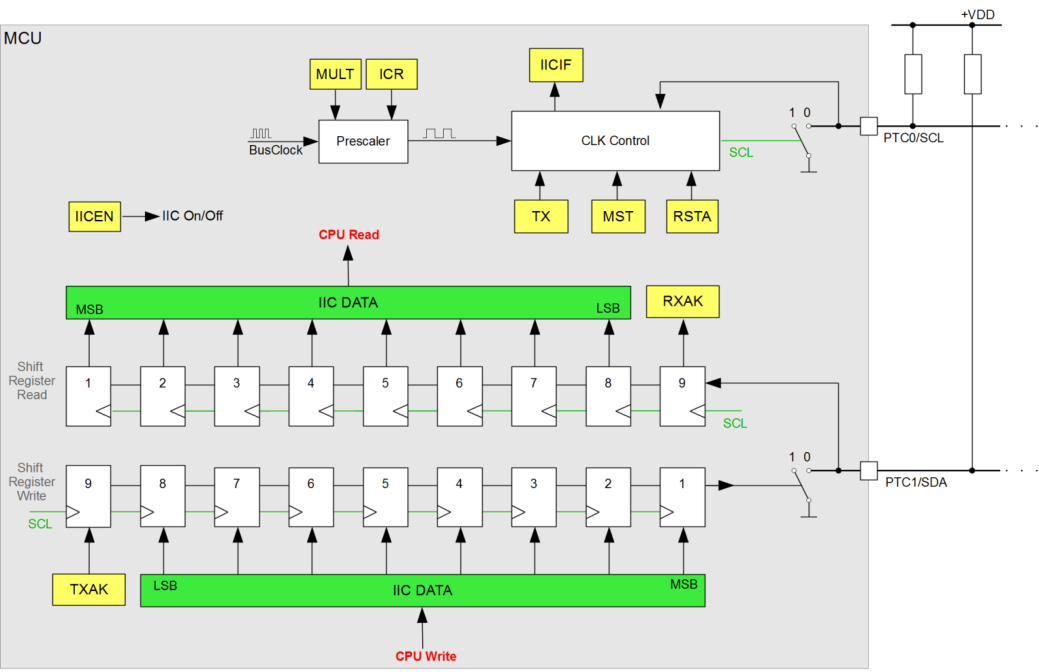
\includegraphics[width=1\textwidth]{../fig/i2c.pdf}
	\caption{Übersicht der I2C Register}
\end{figure}

\newpage
\begin{figure}[h!]
	\centering
	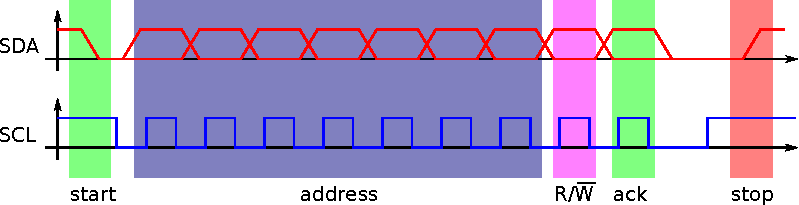
\includegraphics[width=1\textwidth]{../fig/i2c_header.pdf}
	\caption{I2C Header}
\end{figure}

\begin{figure}[h!]
	\centering
	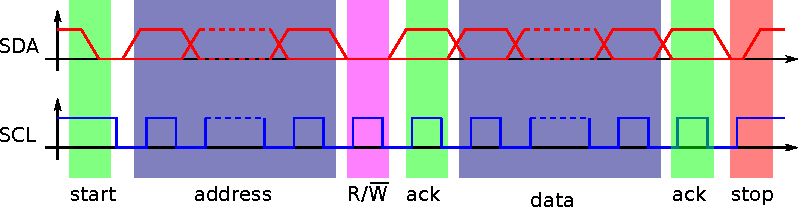
\includegraphics[width=1\textwidth]{../fig/i2c_write.pdf}
	\caption{I2C Write}
\end{figure}

\begin{figure}[h!]
	\centering
	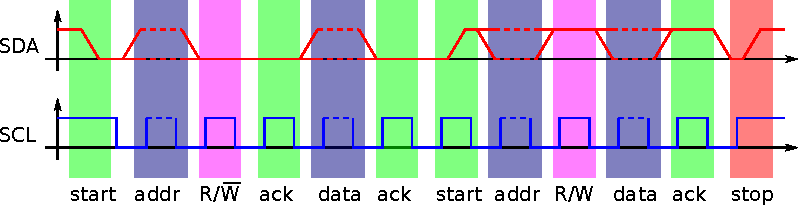
\includegraphics[width=1\textwidth]{../fig/i2c_repeat.pdf}
	\caption{I2C Repeated start}
\end{figure}

\newpage
\subsection{Beispiel}
\lstinputlisting[title=main.c]{../src/i2c_01/Sources/main.c}
\lstinputlisting[title=i2c.h]{../src/i2c_01/Project_Headers/i2c.h}
\lstinputlisting[title=i2c.c]{../src/i2c_01/Sources/i2c.c}
\lstinputlisting[title=qenc.h]{../src/i2c_01/Project_Headers/qenc.h}
\lstinputlisting[title=qenc.c]{../src/i2c_01/Sources/qenc.c}
